\documentclass[utf8,14pt,a4paper,oneside,russian]{book}
\usepackage[14pt]{extsizes}
\usepackage{longtable}
\usepackage{listings}
\usepackage{mathtools}
\usepackage{amsmath}

%===========
%=Кодировка=
%===========
\usepackage[T2A]{fontenc}
\usepackage[utf8]{inputenc}
\usepackage[main=russian, english]{babel}

%===================
%=Разметка страницы=
%===================
\usepackage[left=3cm, right=1cm, top=2cm, bottom=2cm, headheight=14pt, headsep=1cm, footskip=1cm]{geometry}
\pagestyle{plain}
\linespread{1.1} %Межстрочный интервад
\setlength{\parindent}{1.25cm} %Абзацный отступ
\setlength{\parskip}{0em} %Интервал между абзацами
\usepackage{indentfirst}

\usepackage{misccorr}
\usepackage{graphicx}
\usepackage{amsmath, amssymb, amsfonts}

%===========
%=Заголовки=
%===========
\usepackage{titlesec}

\titleformat{\section}{\centering\large\bfseries}{\thesection.}{0.5em}{\MakeUppercase}
\renewcommand{\thesection}{\arabic{section}}
\renewcommand{\sectionmark}[1]{\markright{\thesection.~#1}}
\titlespacing*{\section}{0em}{2em}{1em}

\titleformat{\subsection}{\centering\normalsize\bfseries}{\thesubsection.}{0.5em}{}
\renewcommand{\thesubsection}{\arabic{section}.\arabic{subsection}}
\titlespacing*{\subsection}{0em}{1.25em}{0.5em}

\titlespacing*{\paragraph}{0em}{1.05em}{0.25em}

%============
%=Содержание=
%============
\usepackage{titletoc}
\makeatletter
\renewcommand{\tableofcontents}{\section*{Содержание}\markboth{Содержание}{}\@starttoc{toc}\newpage}
\makeatother
\titlecontents{section}[1.5em]{}{\contentslabel[\thecontentslabel.]{1.5em}}{}{\rule{0.1cm}{0pt}\titlerule*[0.75pc]{.}\contentspage}
\titlecontents{subsection}[4em]{\vspace{0.05em}}{\contentslabel[\thecontentslabel.]{2em}}{}{\rule{0.1cm}{0pt}\titlerule*[0.75pc]{.}\contentspage}

%========
%=Списки=
%========
\usepackage{enumitem}
\makeatletter
\AddEnumerateCounter{\asbuk}{\@asbuk}{м)}
\makeatother
\setlist{nolistsep, topsep=0.375em}
\setenumerate{leftmargin=2cm, labelsep=0em, labelwidth=0.75cm, align=left}
\setitemize{leftmargin=2cm, labelsep=0em, labelwidth=0.75cm, align=left}
\renewcommand{\labelitemi}{--}
\renewcommand{\labelenumi}{\arabic{enumi})}
\renewcommand{\labelenumii}{\asbuk{enumii})}
\renewcommand{\labelenumiii}{--}

%==========================
%=Математические операторы=
%==========================
\DeclareMathOperator{\mob}{Mob}
\DeclareMathOperator{\fix}{Fix}
\DeclareMathOperator{\ord}{ord}

\graphicspath{{pictures/}}
\DeclareGraphicsExtensions{.pdf,.png,.jpg}

\begin{document}

\thispagestyle{empty}
\small
\begin{center}
    
\includegraphics[width=4.55cm]{logo_mirea}\\
    \MakeUppercase{Минобрнауки России}\\[1em]
    Федеральное государственное бюджетное образовательное учреждение\\
    высшего образования\\[0.5em]
    \textbf{<<МИРЭА -- Российский технологический университет>>}\\
    \textbf{РТУ МИРЭА}\\
    \rule{\textwidth}{0.75pt}\\
    Институт Искусственного Интеллекта\\
    Базовая кафедра БК252\\
    
    \rule{\textwidth}{0.75pt}\\[5em]
    \normalsize\MakeUppercase{\textbf{Практическая работа}}\small\\[0.5em]
    По дисциплине <<Системы управления базами данных>>\\[1.5em]
    \begin{tabular}{p{7cm}p{6cm}c}
        Студент группы ККСО-03-19 & Николенко В.О. & \rule{2cm}{0pt}                    \\[-0.5em]
                                  &                & \\[1em]
        Студент группы ККСО-03-19 & Воеводин К.А.  & \rule{2cm}{0pt}                    \\[-0.5em]
                                  &                & \\[1em]
        Студент группы ККСО-03-19 & Носов Г.А. & \rule{2cm}{0pt}                    \\[-0.5em]
                                  &                & \\[1em]
        Студент группы ККСО-03-19 & Базарова Е.O. & \rule{2cm}{0pt}                    \\[-0.5em]
                                  &                & \\[1em]
        Преподаватель             & Колесников С.В.  & \rule{2cm}{0pt}                    \\[-0.5em]
                                  &                & \\[5em]
    \end{tabular}
    \vfill
    Москва -- 2023
\end{center}
\normalsize
\newpage

% Содержание
\tableofcontents

% Первая глава
\newpage
\section{Введение}
Целью этого проекта для курса "Системы управления базами данных" \\
является разработка программы, включающей в себя процессы сбора и обрадотки данных. 
Подробности разработки приведены в этом отчете. Отчёт
включает в себя распределение задач и процессов внутри группы студентов.

Мы начнём с поставленной задачи, разбиения её на этапы, поднимемся на уровень 
реализации логики локальной БД и реализации программного кода, после чего
произведем проверку. 

\newpage
\section{Описание проекта}

\subsection{Цель}

Целью является разработка приложения, которое получающет данные с помощью API,
обрабатывает их и сохраняет в локальную БД. В роли БД будут 2 таблицы, создаваемые
и наполняемые данными в результате работы программы. 

\subsection{Процедура логического проектирования}

В процессе разработки использьзовались такие инструменты как github
 и trello. Каждый из студентов отвечал за конкретные задачи:

 Николенко В. О. - разработка API, её подключение и написание основной части функций вызова.

 Воеводин К. А. - рассчет математической модели и общих параметров БД.

 Носов Г. А. - доработка мат модели и реализация обработки и хранения данных.

 Базарова Е. О. - доработка, тест API и его настройка, составление и написание отчета.

Программа реализована на языке TypeScript на npm-подобном  
пакетном менеджере Yarn. Данные загружаются с помощью API с сайта hltv.org.

Hltv.org - это сайт с подробной информацией о киберспортивных событиях, с подробной
статистикой о игроках, командах, турнирах и т.д. Вокруг киберспорта в 
последние годы сформировалось большое количество внимания, фанатской базы и,
соответсвенно, различных турниров с крупными призовыми наградами и ценными трофеями, попасть на которые
могут либо профессиональные команды, имеющие большие успехи в последних событиях, 
либо малоизвестные команды, которые наравне с сотнями других соревнуются
для получения приглашения на основные турниры, в которых соревнуются 15-20 сильнейших
команд.
Таким образом, формируются популярные команды, сделавшие себе репутацию
и на протяжении нескольких лет могут находиться на слуху, но при этом 
при встрече с менее известным соперником потерпеть поражение.

Для того, чтобы здраво оценивать соревновательную форму той или иной команды,
можно путём сбора и обработки информации, в реальном времени иметь представление
о текущей форме конкретной команды.

\newpage
\subsection{Математическая модель}

Для рассчета формы команд используются несколько критериев:

1. Рейтинг команды со значениями от 0 до 1000 (в таблице обозначен как ranking), рассчитываемый на основе 
числа выиграных турниров, занятого места и важности самих турниров.

2. Текущий уровень формы каждого отдельно взятого игрока (обозначен как rating 2.0)
- основывается на результатах игрока за каждый сыгранный матч по параметрам (kd, avg damage, число раундов взятых командой благодаря этому игроку),
в таблице обозначен как avg2.0 - средее значение данного параметра по команде.

3. Число матчей, сыгранных за последний месяц / полтора / два с половиной 
(в таблице обозначены как ma1, ma1,5, ma2,5) - выясняется сколько матчей было сыграно
за промежуток времени и сколько из них выиграно, делится число побед на число игр в общем.

4. Статистика сыгранных матчей команды, сыгранных ей на конкретной карте. Таким образом,
составляется список карт каждой команды, на которых она имеет лучшие результаты. Информация
по статистике наждой команды на каждой карте находится во второй таблице. 


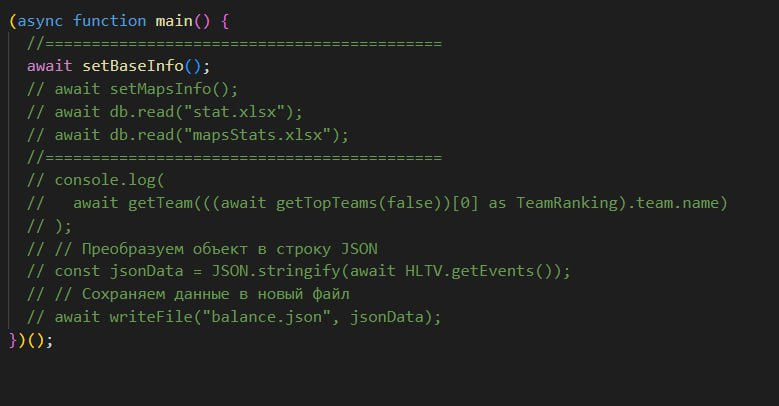
\includegraphics[width=15cm]{main}



Таким образом выглядят вызываемые функции в файле main, за один 
запуск программы мы можем вызвать только одну из них, т. к. сайт 
с исходной информацией содержит ограничение по числу запросов за 
одну сессию. Воизбежание проблем с качеством и скоростью работы
программы было принято решение разделить функции и отдельно запускать 
их с каждым запуском программы.


\newpage
\subsection{Аналитика}

Для анализа статистики игр команд используются данные о 
прошедших матчах на различных картах в течение последних 
2,5 месяцев. Мы использовали рейтинг, который учитывает 
результаты игр, их важность и результаты игр на определенных картах.

Затем мы построили линейную диаграмму, на которой отображены пять 
самых сильных и пять самых слабых команд. Для этого мы отсортировали 
команды по их рейтингу и выбрали пять сильнейших команд и пять команд
со слабыми результатами.

Для определения влияния карты на результаты игры мы использовали 
коэффициент Пирсона, который позволяет оценить силу связи между 
двумя переменными. В данном случае мы сравнивали рейтинг команды 
и результаты ее игр на конкретной карте. Коэффициент Пирсона 
вычисляется по формуле:

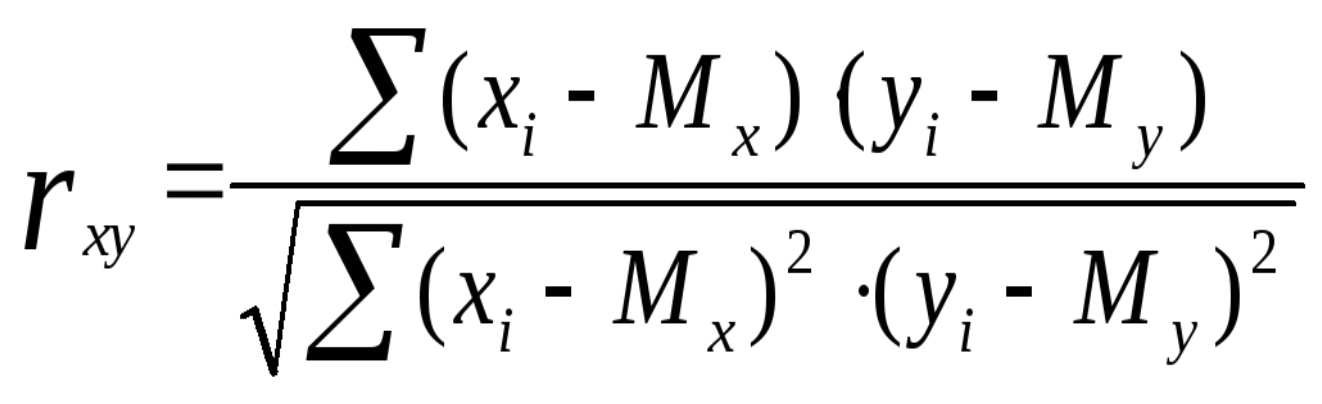
\includegraphics[width=7cm]{form}

где \(x_i\) - рейтинг команды на карте i, \(y_i\) - результаты игр 
команды на карте i, n - количество карт. Коэффициент Пирсона принимает 
значения от -1 до 1, где -1 означает полную отрицательную связь, 
1 - положительную связь, а 0 - отсутствие связи.

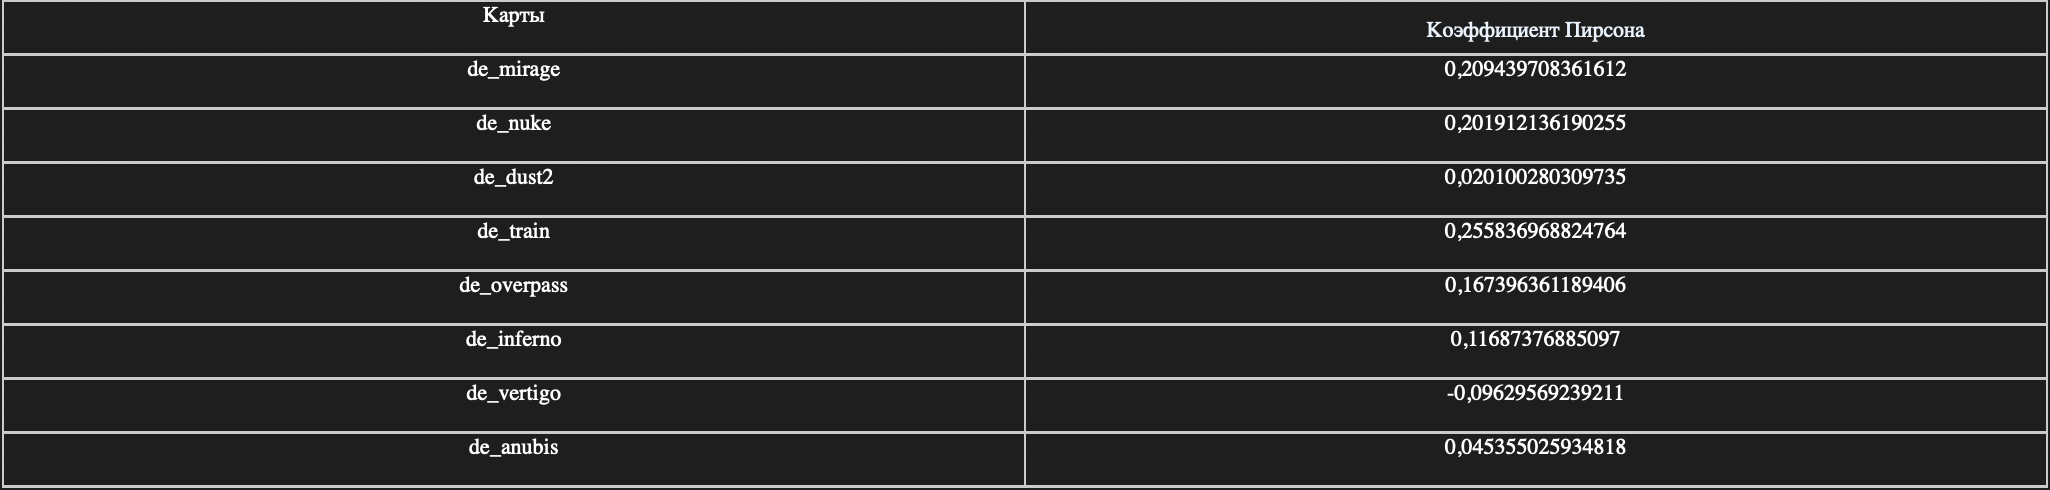
\includegraphics[width=15cm]{table}

Анализ статистики игр показал, что обучаться лучше всего на карте 
de train. Коэффициент Пирсона между рейтингом команды и результатами 
игр на этой карте был выше, чем на других картах, что свидетельствует 
о более сильной связи между этими факторами. Данная карта обеспечивает 
наилучшие условия для развития навыков и стратегий команды, что в свою 
очередь влияет на результаты игр.

На картах de anubis и de dust2 будет сложнее спрогнозировать результаты игр, 
что подтверждается коэффициентом Пирсона, который был ниже, чем на других 
картах. Это свидетельствует о том, что на этих картах результаты игр могут 
быть менее предсказуемыми и менее связанными с рейтингом команды. 
Также было обнаружено, что на карте de vertigo слабые команды могут показывать 
хорошие результаты, что может быть связано с особенностями карты и стратегиями, 
которые используются на ней.

Линейная диаграмма пять самых сильных и пять самых слабых команд показала, 
что разница в рейтинге между самыми сильными и самыми слабыми командами в 
целом не является значительной. Например, на некоторых картах, рейтинг самой 
сильной команды может быть в два или более раза выше, чем рейтинг самой 
слабой команды. Однако, как уже было отмечено, на определенных картах даже 
слабые команды могут показывать хорошие результаты.

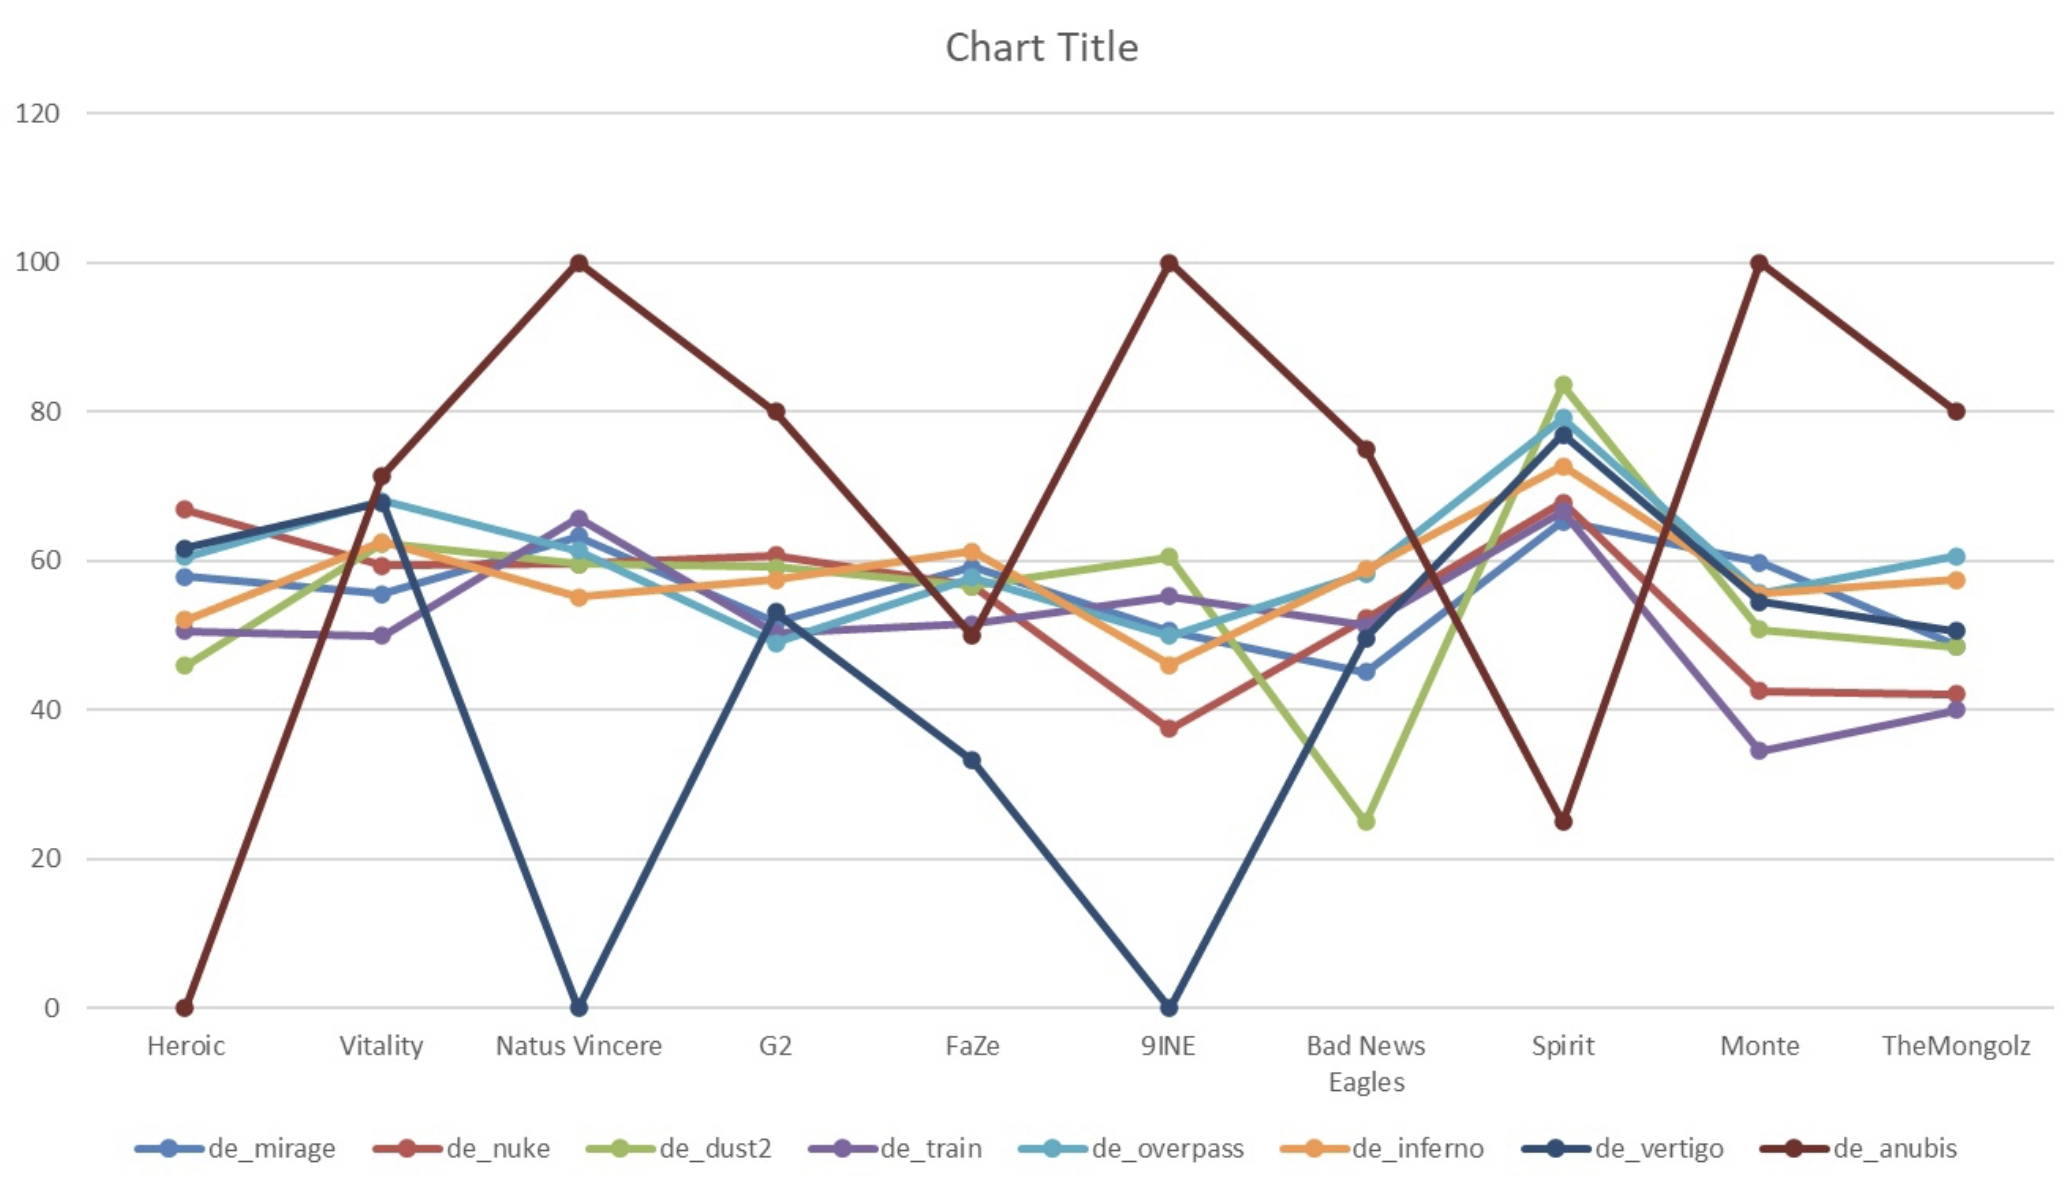
\includegraphics[width=15cm]{graf1}


\newpage
    \section{Практическая реализация проекта}
        \subsection{Архитертура проекта}
        Проект представляет из себя несколько файлов с программным кодом:
        DB.ts - представлен классом DB который имеет 2 поля: конструктор и
         функции, 2 публичные переменные класса - имя файла и область данных, 
         которая будет записана в виде new Excel.Workbook(), для этого использует 
         библиотека exceljs.
         По итогу получаем 2 следующих таблицы:
         \begin{center}
         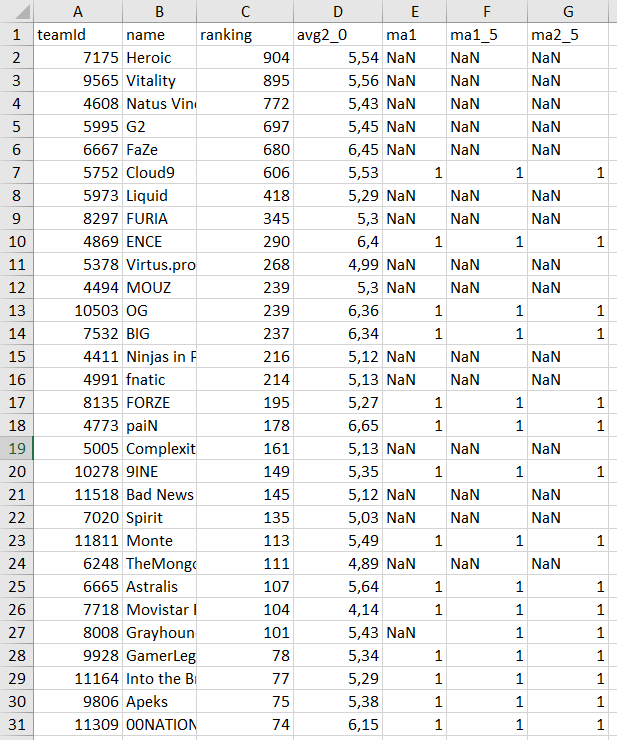
\includegraphics[width=9cm]{tbl2}
         
         Рис.1. Таблица со статистикой команд.

         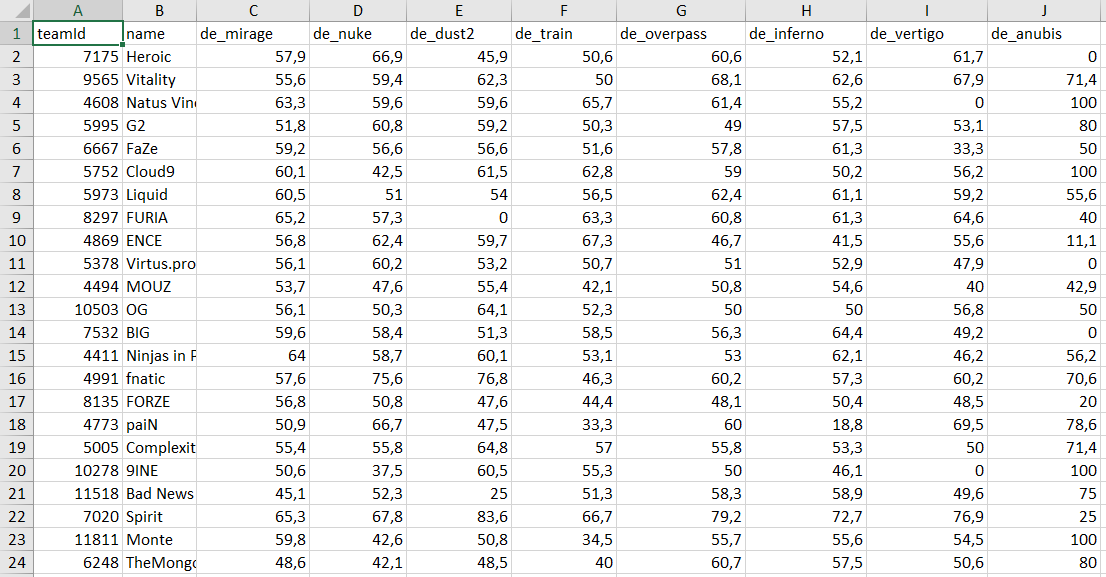
\includegraphics[width=14cm]{tbl1}

         Рис.2. Таблица со статистикой побед команд по картам.
        \end{center}

        HLTV-HANDLER - Представлен набором функций/типов/переменных, которые видны извне и к которым можно обращаться из других программ/модулей. Они в свою очередь обращаются к hltv api и подтягивают базовые данные с сайта, которые впоследствии обрабатываются внутри нашей программы и заносятся в таблицу в нужной нам форме.

        В результате до записи в таблицу имее возможность вывода 
        в терминал следующие параметры объектов:
        
        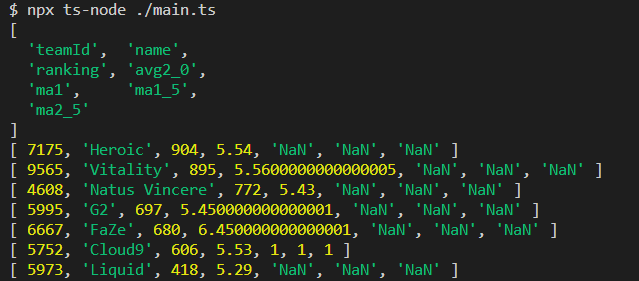
\includegraphics[width=15cm]{term1}
        \begin{center}
          Рис.3. Полученные данные для записи в таблицу 1.
        \end{center}

        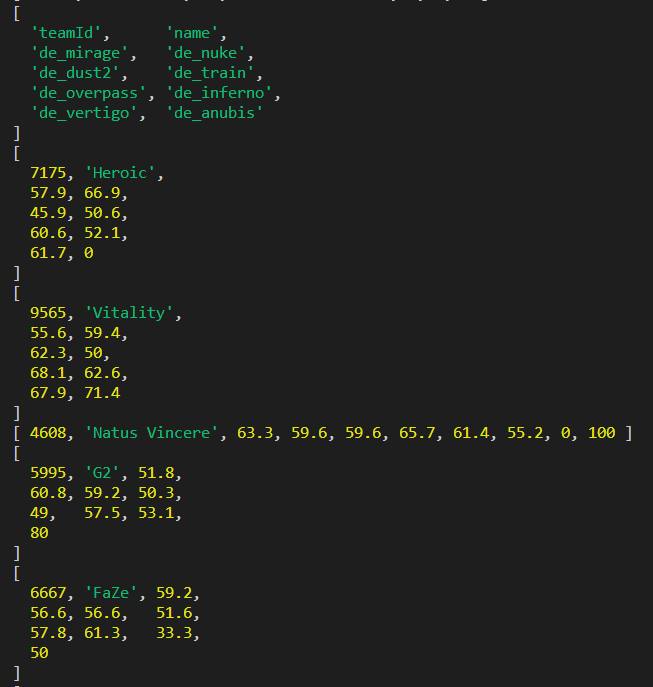
\includegraphics[width=10cm]{term2}
        \begin{center}
          Рис.3. Полученные данные для записи в таблицу 2.
        \end{center}

        \newpage
        \subsection{Программный код}
        \begin{lstlisting}
            public addRaw<T>(sheet: string, entity: T) {
    let worksheet = this.workbook.getWorksheet(sheet);

    if (typeof worksheet === "undefined") {
      worksheet = this.workbook.addWorksheet(sheet);

      worksheet.columns = [
        ...Object.keys(entity as Object).map((x: any) => {
          if (x == "id1_id2") {
            return { header: x, key: x, width: x.length + 25};
          }
          return { header: x, key: x, width: x.length + 5};
        }),
      ];
    } else {
      // comparison of type of entity and existing columns
      // spoiler: must be equal
      let k: keyof typeof entity;
      for (k in entity)
        if ((worksheet._keys[k] as String) == (entity[k]
         as String))
          throw "Incompatible types";
    }

    worksheet.addRow(entity);
  }
\end{lstlisting}

  Функция addRaw принимает некую сущность произвольного типа, в нашем случае это объект:
  
  \begin{lstlisting}
  interface teamInfo {
  teamId: number;
  name: string;
  ranking: number;
  avg2_0: number;
  ma1: number;
  ma1_5: number;
  ma2_5: number;
  }
\end{lstlisting}
И преобразует её в строку, для каждого элемента выделен свой столбец.

Впоследствии эта строка записывается в область данных, которая была описана выше.

\begin{lstlisting}
    public showWorkbook(workbook?: Workbook) {
    let currentWB = typeof workbook === "undefined" ?
     this.workbook : workbook;

    for (let i = 0; i < currentWB.worksheets.length; i++) {
      for (let j = 1; j <= currentWB.worksheets[i].rowCount;
       j++) {
        console.log(currentWB.worksheets[i].getRow(j)
        .values.slice(1));
      }
    }
  }
  \end{lstlisting}

  Функция showWorkbook выводит нынешнее состояние области данных, которую мы заполниоли при помощи addRaw.

  Функции read/write:
  \begin{lstlisting}
    public async write(fileName: string) {
    await this.workbook.xlsx.writeFile(fileName);
    console.log(`File {fileName} is written`);
  }

  public async read(fileName: string) {
    const workbook = await this.workbook.xlsx
    .readFile(fileName);
    this.showWorkbook(workbook);
  }
\end{lstlisting}

Write  - записывает наш workbook в файл с именем, в случае, если файла нет, то создаёт его.
read - читает из файла с заданным именем, если файла нет - выдаёт ошибку.

\begin{center}
\end{center}

\newpage
\end{document}